\chapter{Úvod}
Zpracování řeči hraje v~dnešní době důležitou roli v~mnoha rozličných oborech. Mezi jeden z~hlavních úkolů bezesporu patří separace zdrojů v~zaznamenaném signálu, který může být složen ze signálů N mluvčích, ale i nechtěného hluku okolí. Vyřešení problému je předpoklad k~dalším úkonům jako identifikace konkrétního mluvčího nebo třeba přepis konverzace na text. Se stále se zrychlujícím vývojem počítačů a s~jejich zvyšujícím se výkonem se do popředí dostávají metody zpracování řeči založené na neuronových sítích, které v~mnoha ohledech předčily ostatní algoritmy strojového učení.

Separace mluvčích v~časové doméně dosahuje mimořádných výsledků v~porovnání s~dosavadními metodami  založenými na převodu signálu z~časové domény do frekvenční domény pomocí algoritmu STFT (Short--Time Fourier Transformation). Taková reprezentace signálu není optimalizovaná pro separaci řeči a nemusí pro tento úkol být optimální. V~architektuře, která je navržena v~referenční studii s názvem \textbf{TasNet: Surpassing Ideal Time-Frequency Masking for Speech Separation}\cite{luo2018convtasnet}, je vstupní signál převeden do nezáporné reprezentace, která je optimální pro extrakci jednotlivých mluvčích. Silnou stránkou systému je hluboká architektura sítě, která lépe modeluje dlouhodobé závislosti v~signálu. Zárověň se ale musí vypořádat s~problémy, které hluboké neuronové sítě mohou přinášet.

Úkolem této práce je nastudovat si problematiku neuronových sítí a jejich základní principy, seznámit se problémem separace mluvčích pomocí neuronových sítí a následně implementovat síť podle architektury TasNet pro separaci mluvčích v~časové doméně, která byla navržena a popsána ve studii\cite{luo2018convtasnet}. Poté tuto neuronovou síť natrénovat s~různými kombinacemi hodnot hyperparametrů, které ovlivňují velikost sítě  její vlastnosti, a nakonec porovnat přesnost a kvalitu separace mezi jednotlivými, různě velkými sitěmi a mezi výsledky studie. Přesnost a kvalita separace bude vypočítána pomocí metrik určených k hodnocení kvality řečového signálu. Sítě budou testovány a vyhodnocovány na testovací množině jednokanálových směsí dvou mluvčích.

Text je rozdělen na několik kapitol, které postupně pokrývají různé logické celky. V kapitole \ref{separace} je popsán problém separace mluvčích a dosavadní přistupy k jeho řešení. Kapitola \ref{neuronovky} se zabývá základními vlastnostmi a principi neuronových sítí. V kapitole \ref{tasnet} je věnována architektuře TasNet, kterou se moje práce zabývá. Dále kapitola \ref{implementace} popisuje implementaci sítě a pomocných nástrojů a nakonec v kapitole \ref{experimenty} jsou experimenty a vyhodnocování přesnosti sítě.


%----------------------------------------------------------------------------------------------------------------------------------------------------------------------
\chapter{Separace mluvčích}
\label{separace}
Živočichové mají vrozenou schopnost zaměřit se na jeden konkrétní zvuk, zatímco všechny ostatní dokážou potlačit. Naučit ale této dovednosti počítač se ukázalo jako obtížný úkol, který je překážkou ASR (\textit{automatic speech recognition}) systémům v rozsáhlejším nasazení do běžného života. Tento problém se nazývá koktejl párty. Vyřešení tohoto problému, tedy separování zdrojů, umožňuje širokou aplikaci v oblasti zpracování řeči, jako  přepis konverzací na text, ovládání počítače hlasem, používání hlasových asistentů či identifikace konkrétního mluvčího v prostředí s mnoha současně mluvícími lidmi.

\section{Koktejl párty efekt}
Tento problém se nejlépe dá popsat jako schopnost soustředit se na jeden konkrétní zdroj zvuku z mnoha souběžných zdrojů jako hudba, konkrétní hudební nástroj, řeč dalších lidí či okolní zvuky, a přepínat mezi nimi dynamicky pozornost. 

\todo{vzniklo pro jeho vyreseni hafo altofirmu, ktere dosahovaly nejakych vysledku. jeho vyresenim by se mohlo pouzivat asr na prepis reci an text a pod. Nejlepsich vysledku dosahly hluboke neuronove site.}


\section{Metody pro separaci jednokanálových nahrávek}
Pro separaci zdrojových signálů z nahrávek směsí existuje mnoho algoritmů založených na zpracování signálů, z nichž asi nejznámější jsou CASA (\textit{computational auditory scene analysis})\todo{ref?} a NMF (\textit{non-negative matrix factorization}) \todo{ref?}, používané pro separaci jednokanálových nahrávek. V posledních letech se do popředí dostaly přistupy založené na hlubokých neuronových sítích, které předčily svou přesností a výkonností dosavadní algoritmy. Pro separaci vícekanálových nahrávek se používají metody \textit{beamforming} nebo state--of--the--art \textit{Multi-channel blind source separation}, které ale jsou nad rámec této práce. Tato kapitola shrnuje některé metody pro řešení separace, které jsou zmíněny v článku\cite{speechseparation}.


\subsection{CASA -- computational auditory scene analysis}
Metoda CASA je založena na procesu v lidském mozku, který separuje zdroje ze směsi mluvčích a simuluje vysokoúrovňové chování lidského sluchu. Pro separaci jsou většinou manuálně navrhnuta segmentační pravidla pro operování nad nízkoúrovňovými příznaky k odhadu časově frekvenční (\textit{T--F}) masky, která izoluje komponenty signálu jednotlivých mluvčích a následně je použita pro rekonstrukci všech zdrojů.
\todo{Hodit sem teda ty zdroje jako v 3.1 pro ASA, CASA a pod? jak jsou tam asi 3 po sobe?}

Přestože tato metoda byla i nadále rozvíjena, tak má mnoho nevýhod jako špatnou generalizaci v důsledku manuálního vytváření pravidel, nemožnost automatického učení z dat nebo nemožnost použití na separaci jiných zdrojů než je lidská řeč, které značně omezují její použití v mnoha reálných případech.



\subsection{NMF -- non-negative matrix factorization}
Nezáporná maticová faktorizace (\textit{NMF}) \todo{[(Lee and Seung, 2001)]} patří mezi daty řízené metody a je založena na předpokladu, že struktura spektrogramu může být reprezentována malým počtem bází.

Pro NMF platí

\begin{equation}
  Y = \sum{s}W_sH_s
\end{equation}

kde každý zdroj $s$ je modelován aproximací nízkého řádu nezápornými maticemi $W_s$, která reprezentuje slovník a $H_s$, která reprezentuje aktivační funkci. Ty jsou sečteny a dohromady tvoří výslednou směs $Y$.

Metoda prochází trénovací a testovací fází.
V trénovací fázi je každý zdroj dekomponován a mapován na množinu bází a aktivací a tím je zformován slovník $W$ pro tento zdroj.
V testovací fázi jsou naučené slovníky jednotlivých zdrojů $s$ spojeny do jednoho, který dále není upravován. Následuje optimalizace aktivační matice $H$ pro každý zdroj. Každý zdroj je následně ze směsi rekonstruován s použitím výsledných bází a aktivací.

\begin{figure}[H]
    \centering
    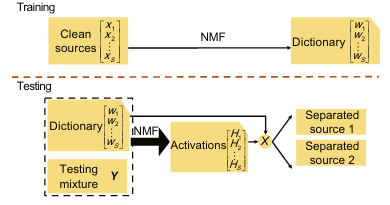
\includegraphics[scale=0.6]{obrazky-figures/nmf.png}
    \caption{\label{fig:nmf}Znázornění trénovací a testovací fáze. Obrázek byl inspirován \cite{speechseparation}}
\end{figure}

Stejně jako metoda CASA, i tato má mnoho nevýhod, které omezují její použití pro řešení reálných problémů separace.



\subsection{Hluboké neuronové sítě}
Nejlépe si při řešení problému koktejl párty vedou postupy založené na hlubokém učení a neuronových sítích.
Metody převáděly směs do časově--frekvenční reprezentace znázorněné na obrázku \ref{fig:spektrum} pomocí STFT (\textit{short time fourier transformation}).

\begin{figure}[H]
    \centering
    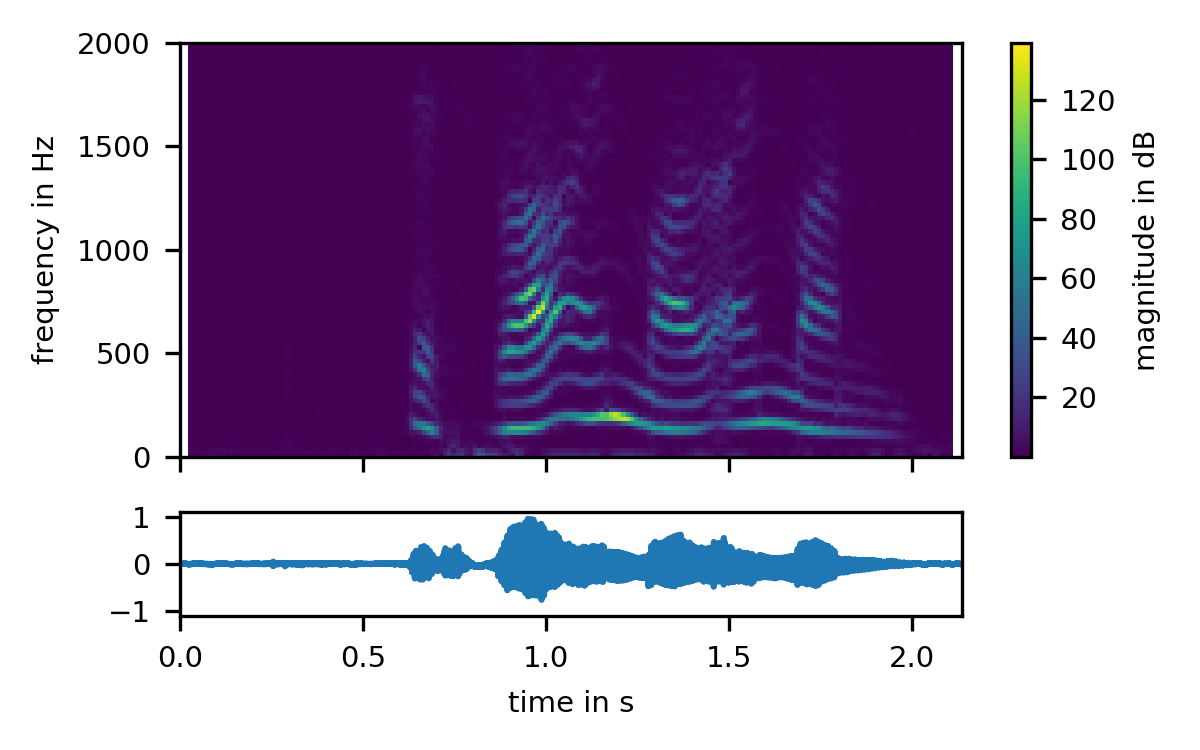
\includegraphics[scale=0.6]{obrazky-figures/spektrum.png}
    \caption{\label{fig:spektrum}Časově--frekvenční reprezentace řeči, neboli spektrum}
\end{figure}




\section{Vyhodnocovací metriky}
Pro vyhodnocení kvality separace se používají různé metriky. Jejich volba závisí na řešeném problému.


\subsection{Signal--to--noise ratio}
Nejzákladnější metrika pro určení kvality separace je signal--to--noise ratio (SNR), která porovnává zastoupení chtěného signálu a šumu v pozadí a je definována jako poměr energie originálního (ideálního) signálu a energie rozdílu mezi originálním a rekonstruovaným signálem.

\begin{equation}
  SNR = \frac{E_s}{E_N}
\end{equation}

Výsledný poměr často bývá vyjádřen v decibelech jako

\begin{equation}
  SNR(dB) = 10log_{10}\frac{E_s}{E_N}
\end{equation}

kde kladná SNR hodnota udává, že zastoupení signálu je větší, než zastoupení šumu \todo{citovat https://labrosa.ee.columbia.edu/~dpwe/pubs/Ellis04-sepeval.pdf}.



\subsection{SDR -- Source Distortion Ratio}
SDR je jedna z nejznámějších metrik pro měření kvality řečového signálu.


\subsection{PESQ -- Perceptual evaluation of speech qualit}
Procentuální vyhodnocení kvality řeči (PESQ\cite{pesq-itut}) je standardizovaná metrika pro vyhodnocování kvality řeči. Jeho hodnota se pohybuje od -0.5 do 4.5 s tím, že vyšší hodnota znamená lepší procentuální kvalitu\cite{DBLP:journals/corr/abs-1901-09146}.


\subsection{STOI}


Bylo navrženo mnoho konvenčních přístupů a metod pro řešení problému koktejl párty a s ním spojené separace mluvčích, ale většina z nich nedosahuje dostatečné přesnosti nebo výkonu k použití v reálných situacích. Přístupy založené na hlubokém učení a neuronových sítích předčily dosavadní techniky jak v přesnosti, tak ve výkonu, což umožňuje jejich nasazení v běžném životě.


%----------------------------------------------------------------------------------------------------------------------------------------------------------------------
\chapter{Neuronové sítě}
\label{neuronovky}
V~dnešní době zažívají neuronové sítě díky výkonosti počítačů velký rozmach. Jejich využití prostupuje skrze mnohé vědní obory a dokáží řešit celou řadu problémů, ve kterých dosahují výborných výsledků, které zdaleka předčily dosavadní postupy. 

Neuronové sítě (\textit{artificial neural networks}) jsou výpočetní model, který je inspirovaný strukturou lidského mozku, ve kterém je obrovské množství propojených a komunikujících neuronů. Ty se skládají ze vstupních dendridů, výstupních axonů a samotného těla neuronu. Na základě vnitřního potenciálu a vstupních hodnot je po přesažení prahové hodnoty neuron vybuzen a je vyslán signál na výstupní axon. Signál je nakonec předán dalším neuronům skrze jejich vstupní dendridy\cite[p.~65--66]{mitdeeplearning_small}.

Účelem neuronové sítě je naučit se plnit zadanou úlohu. Rozdíl oproti běžným algoritmům je ale ten, že způsob, jakým síť má problém řešit, není explicitně naprogramován, ale je postupně naučen. Základní způsoby učení jsou s~učitelem (\textit{supervised}) a bez učitele (\textit{unsupervised}). 

\textbf{Učení s~učitelem}, pod které spadá i tato práce, spočívá v~mapování vstupních dat na data výstupní na základě vzorových příkladů dvojic vstup--výstup. Množině takových dvojic se říká trénovací dataset. Další vlastností trénovacích dat určených pro učení s učitelem, je jejich označení (\textit{label}).

Mezi problémy, které se dají řešit neuronovými sítěmi patří klasifikační a regresní problémy. Konkrétní příklad z~oblasti klasifikace může být rozpoznávání objektů na obraze, psaného písma nebo detekce obličejů na videu, ale i mnohé aplikace ve zpracování řeči. Některé z problémů lze řešit sítí, která se skládá z jednotek neuronů, zatímco složitější problémy vyžadují mnohem větší kapacitu sítě a ta pak může obsahovat i tisíce neuronů.

Upravovat samotnou strukturu a chování neuronové sítě lze pomocí jejích hyperparametrů, což jsou parametry určující nastavení neuronové sítě a trénovacího algoritmu. Tyto parametry musí být určeny před začátkem trénování a většinu nelze později měnit. Mohou určovat kapacitu modelu, velikost záběrného pole, velikost filtrů, ale i regulovat samotný proces učení nastavením počtu epoch, po které se model má učit, nebo také počet dat předaný v jedné dávce (tzv. \textit{minibatches}) během učení sítě.


\section{Organizace feedforward sítí}
Feed forward neuronové sítě (\textit{Multi Layer Perceptron -- MLP}) jsou typ umělých neuronových sítí, kde se nevyskytují cykly ve výpočetním grafu, tedy zpětná propojení vrstev, takže informace se pohybuje pouze jedním směrem, od vstupní vrstvy přes skryté vrstvy až po vrstvu výstupní. Sítě, které obsahují cykly, se nazývají rekurentní. Rozdíl znázorňuje obrázek \ref{fig:netcomparison}.

\begin{figure}[H]
    \centering
    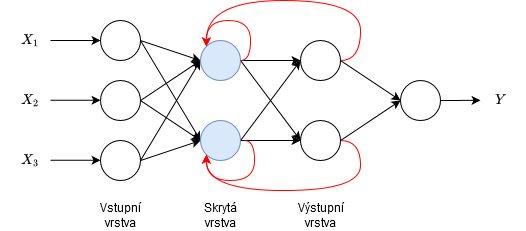
\includegraphics[scale=0.5]{obrazky-figures/feedforward_vs_recurrent.png}
    \caption{\label{fig:netcomparison}Příklad grafu feed forward sítě a rekurentní neuronové sítě. Lze si všimnout orientace šipek u~feed forward sítě, které směřují pouze jedním směrem, zatímco u~rekurentní sítě šipky směřují i k~předešlým uzlům grafu\cite{FFandRecNN}.}
\end{figure}

Struktura neuronové sítě je organizována do vrstev, které se skládají z~neuronů. Feedforward síť je tvořena třemi typy vrstev (viz obrázky \ref{fig:netcomparison} a \ref{fig:mlp}). Vstupní vrstva slouží k~předání hodnot do sítě, ale nijak tyto hodnoty nemodifikuje. Nezměněné jsou zkopírovány do první skryté vrstvy. Následují skryté vrstvy, z~nichž poslední je napojena na výstupní vrstvu. Ta má obvykle méně neuronů než předešlé vrstvy a hodnoty na výstupu mohou představovat třídy, do kterých má být klasifikován vstup v případě klasifikátorů, nebo predikce hodnot na základě vstupních dat v případě regrese. S~počtem jednotlivých vrstev souvisí pojem hloubka sítě, která je rovna počtu všech vrstev neuronové sítě od vstupní až po výstupní vrstvu. Pojem \todo{uvozovky lepe} "hluboká neuronová síť" označuje takovou síť, která má dvě nebo více skrytých vrstev. Existuje mnoho typů vrstev, například plně propojené, pooling, s~přeskočením nebo vrstvy konvoluční.

\begin{figure}[H]
    \centering
    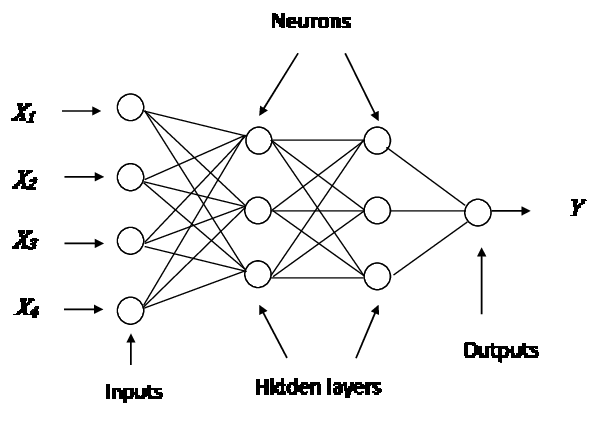
\includegraphics[scale=1.3]{obrazky-figures/mlp.png}
    \caption{\label{fig:mlp}Schéma neuronové sítě, která má 2 skryté vrstvy}
\end{figure}


\section{Umělý neuron}
Základní stavební jednotka neuronových sítí je umělý neuron (\textit{artificial neuron}) (viz obrázek \ref{fig:neuron}). Tento model je založen na principu reálných neuronů, které se nacházejí v~organizmech. Umělý neuron obsahuje libovolně mnoho vstupních propojení, přes které se mu předávají data v~podobě vstupního vektoru $\overrightarrow{x} = [x_1, x_2, \dots, x_n], x_n \in \mathbb{R}$. Sám neuron obsahuje hodnotu bias $b \in \mathbb{R}$ a vektor vah $\overrightarrow{w} = [w_1, w_2, \dots, w_n], w_n \in \mathbb{R}$, jenž je upravován během trénování neuronu.

Výstupní hodnota závisí na vstupních datech, aktuálním vnitřním stavu (hodnoty vah a biase) a na zvolené aktivační funkci. Vstupní hodnoty jsou váhovány, což znamená, že každá vstupní hodnota je vynásobena s~váhou na daném vstupním spojení. S~použitím definovaných vektorů lze napsat, že vstupní vektor je vynásoben s~vektorem vah.

\begin{figure}[H]
    \centering
    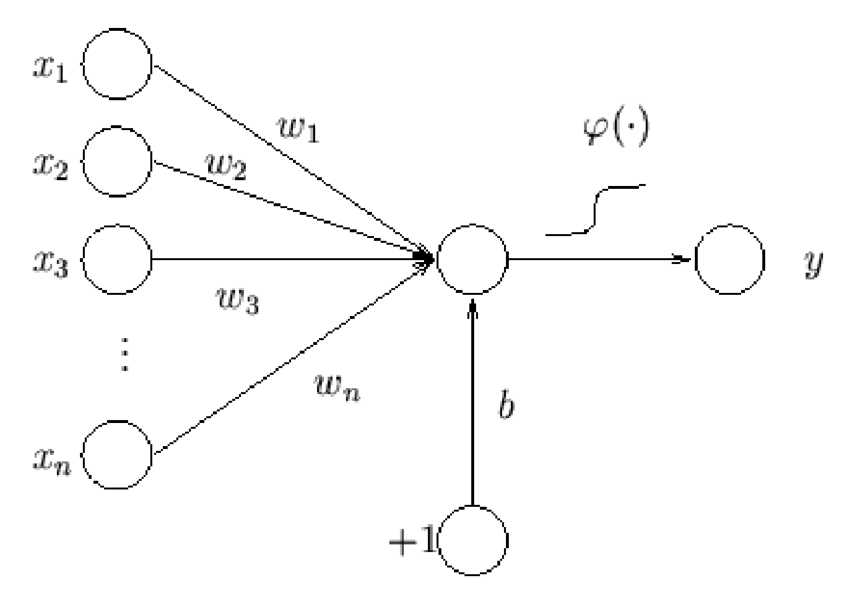
\includegraphics[scale=0.35]{obrazky-figures/perceptron.png}
    \caption{\label{fig:neuron}Schéma umělého neuronu}
\end{figure}

Hodnota bias $b$, která je přičtena k~sumě násobků vah a vstupních hodnot, je prahová hodnota modifikující dobu, kdy se aktivuje neuron a změní svůj výstup. Matematicky to znamená, že s~grafem aktivační funkce horizontálně pohybuje doleva nebo doprava v~závislosti na tom, je-li hodnota biasu pozitivní nebo negativní. Toto posunutí je znázorněno na obrázku \ref{fig:bias}. V~závislosti na řešeném problému může být žádoucí, aby i hodnota bias byla modifikována během učení společně s~ostatními váhami. V~opačném případě je hodnota nastavena pevně na nějakou konstantní hodnotu, obvykle na hodnotu jedna.

\begin{figure}[H]
    \centering
    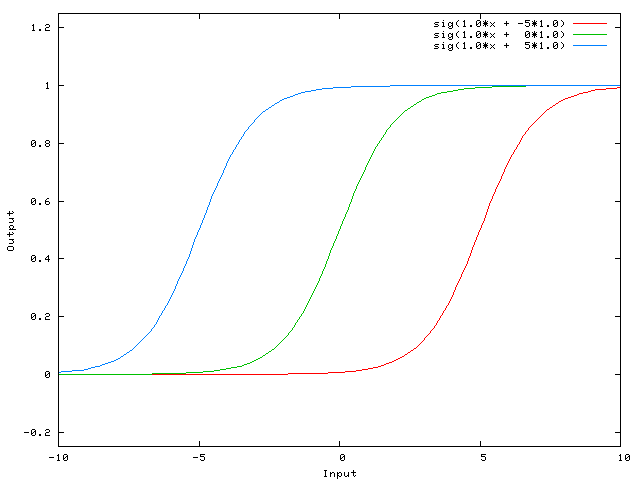
\includegraphics[scale=0.4]{obrazky-figures/bias.png}
    \caption{\label{fig:bias}Vliv hodnoty bias na aktivační funkci}
\end{figure}




Výstup neuronu se vypočítá jako
\begin{equation}
	y = f\Big((\sum_{k=1}^n w_kx_k) + b\Big)
\end{equation}
kde $f$ je aktivační funkce, $x_k \in \mathbb{R}$ je vstupní hodnota, $w_k \in \mathbb{R}$ je váha, kterou se vstupní hodnota vynásobí a $b \in \mathbb{R}$ je hodnota bias.


\section{Aktivační funkce}
Aktivační, neboli prahová funkce, určuje výstupní hodnotu neuronu. Funkce se vybírá na základě problému, který se má neuronová síť naučit řešit. Správná volba aktivační funkce vede k~lepší konvergenci učení sítě. Naopak špatná volba může vést ke stále větší odchylce od správného řešení -- může divergovat. Povaha problému může vyžadovat specifické vlastnosti aktivační funkce - lineární nebo nelineární. Pro nestandardní problémy je obvykle potřeba experimentálně zjistit, která funkce bude nejlépe vyhovovat danému problému. 

Pokud by veškeré aktivační funkce v~modelu byly lineární, tak celkové mapování sítě by bylo omezeno pouze na lineární mapování vstupu na výstup. Reálné problémy ale lineární obvykle nejsou a v~případě pokusu modelovat takovým modelem nelineární vztahy by vedlo k~velice nepřesným výsledkům, který by byl zapříčiněn podučením (\textit{underfitting}), což znamená, že model, který se učí zakódovat nějaký vzor v~datasetu, je příliš jednoduchý. Proto je potřeba zavést do modelu i nelineární aktivační funkce, které tento problém řeší\cite[p.~77--78]{mitdeeplearning_small}.

Z~pohledu učení je také důležité, aby aktivační funkce byla diferencovatelná. To umožňuje použití učících metod založených na výpočtu gradientu, jako je algoritmus backpropagation.



\subsection*{Sigmoid}
\begin{equation}
  f(x) = \frac{1}{1+\exp(-z)}
\end{equation}

\todo{popsat}

\begin{figure}[H]
    \centering
    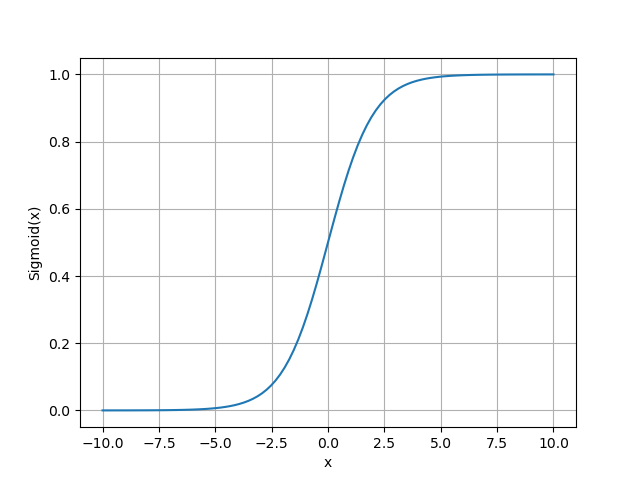
\includegraphics[scale=0.18]{obrazky-figures/sigmoid.png}
    \caption{\label{fig:sigmoid}Graf aktivační funkce sigmoid}
\end{figure}



\subsection*{Softmax}
\begin{equation}
  f(x) = \frac{1}{1+\exp(-z)}
\end{equation}

\todo{popsat}

\begin{figure}[H]
    \centering
    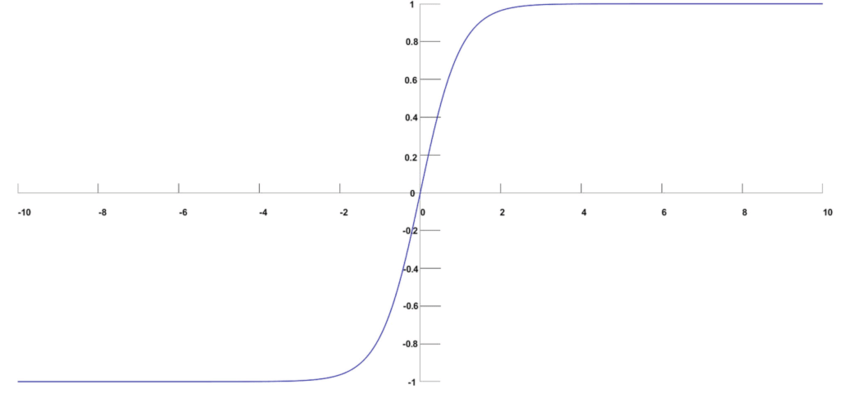
\includegraphics[scale=0.35]{obrazky-figures/softmax.png}
    \caption{\label{fig:softmax}Graf aktivační funkce softmax}
\end{figure}




\subsection*{ReLU}
Rectified Linear Unit je nejčastěji používaná aktivační funkce. Vyžaduje-li neuronová síť nějakou nelinearitu, je ReLU pro většinu případů ideální. Pro každou zápornou hodnotu $x$ vrací $0$ a pro kladnou hodnotu $x$ vrací tutéž hodnotu $x$, jak udává rovnice 
\begin{equation}
   f(x)=max(0,x)
\end{equation}

\begin{figure}[H]
    \centering
    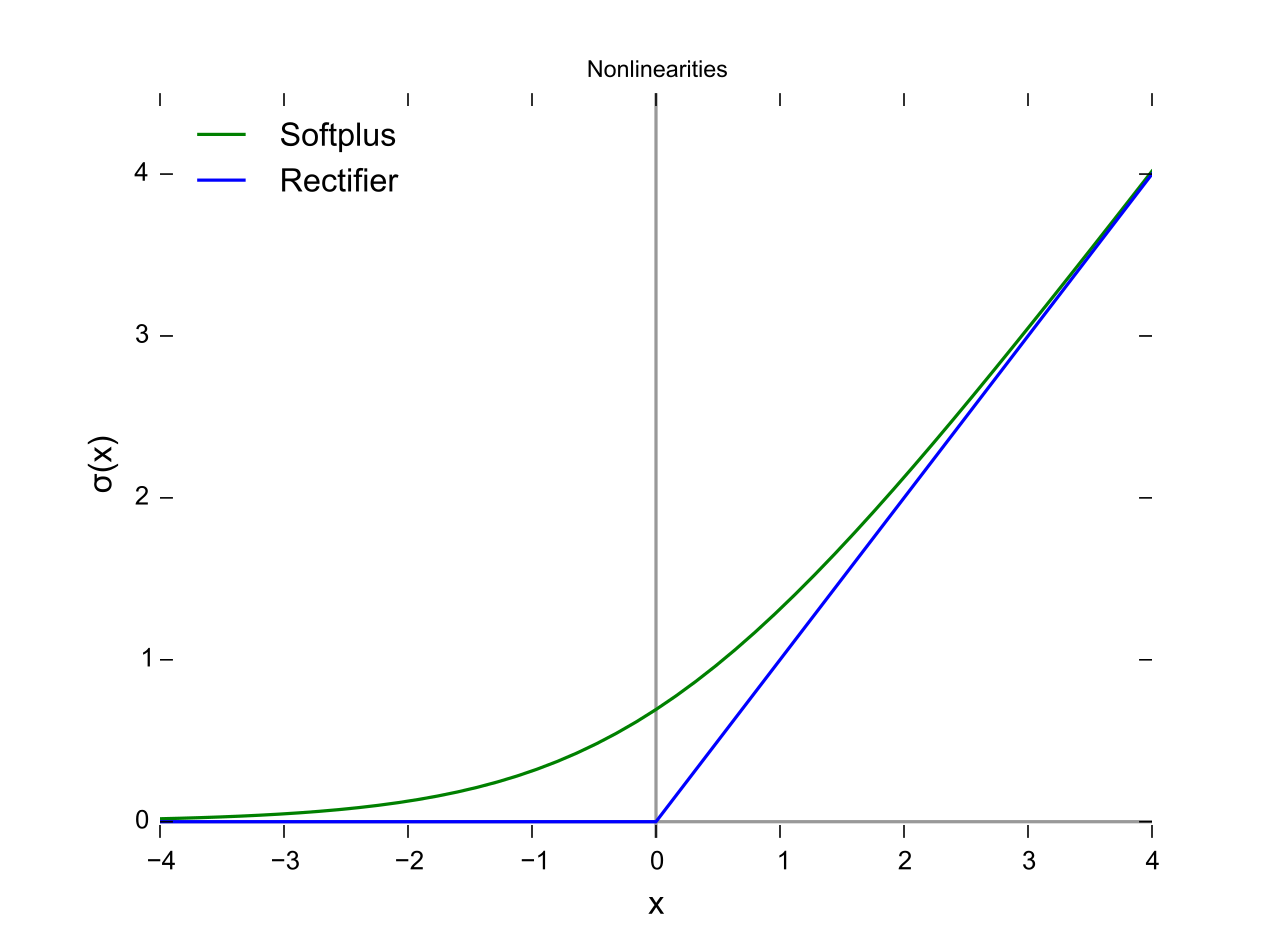
\includegraphics[scale=0.2]{obrazky-figures/ReLU.png}
    \caption{\label{fig:relu}Graf aktivační funkce ReLU}
\end{figure}




\subsection*{PReLU}
Parametrizovaná ReLU je nelineární aktivační funkce, která se používá v~případě, že chceme produkovat na výstup malý nenulový gradient i v~případě záporné vstupní hodnoty $x$. V~tom případě je vstupní hodnota vynásobena parametrem $\alpha$ a to představuje výsledek. Parametr $\alpha$ se společně s~ostatními váhami učí během učícího procesu.
\begin{equation}
  f(x) =
  \begin{cases}
    x & \text{if } x \geq 0 \\
    {\alpha}x & \text{if } x < 0
  \end{cases}
\end{equation}

\begin{figure}[H]
    \centering
    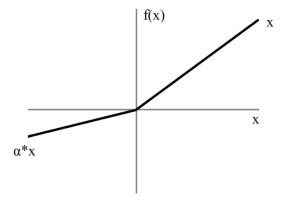
\includegraphics[scale=1.4]{obrazky-figures/prelu.jpg}
    \caption{\label{fig:prelu}Graf aktivační funkce PReLU}
\end{figure}


\section{Lineárně separovatelná data}
Síť složená z~jediného neuronu by byla omezena pouze na klasifikaci lineárně separovatelných dat. To jsou taková data, která lze rozdělit, existuje-li alespoň jedna přímka v~rovině taková, že na jedné straně přímky jsou všechna data klasifikována do první třídy, a na druhé straně data klasifikována do třídy druhé, jak lze vidět na obrázku \ref{fig:linear_separable}.

\begin{figure}[H]
    \centering
    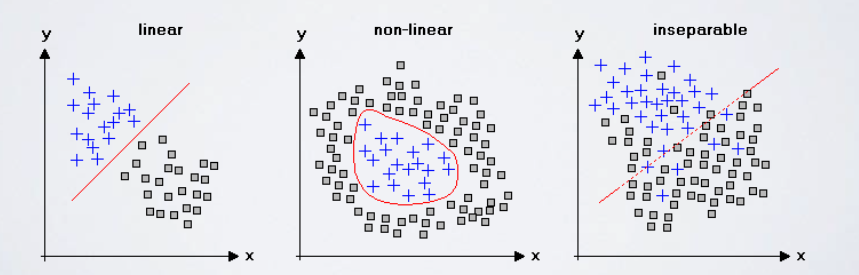
\includegraphics[scale=0.38]{obrazky-figures/linear_separable.png}
    \caption{\label{fig:linear_separable}Lineárně separovatelná (vlevo) a neseparovatelná (vpravo) data} 
\end{figure}

Mějme množinu dat, kterou tvoří dvě rozdílné třídy objektů $\Omega_1, \Omega_2 \subset \mathbb{R}^m$. Třídy jsou lineárně separovatelné, jestliže existuje $w \in 
\mathbb{R}^m$ a $\theta \in \mathbb{R}$ takové, že 
\begin{equation}
   \forall x \in \Omega_1 : x^Tw > \theta
\end{equation}
\begin{equation}
   \forall x \in \Omega_2 : x^Tw < \theta
\end{equation}

Problém lze zobecnit tak, že řešením bude separace tříd pomocí hyper roviny v~prostoru $\mathbb{R}^m$, jak zachycuje obrázek \ref{fig:hyperplane_separable}
\cite{linearseparability}.

\begin{figure}[H]
    \centering
    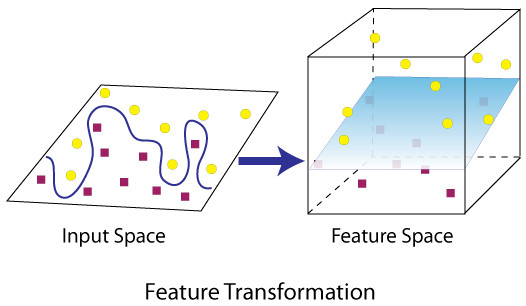
\includegraphics[scale=0.8]{obrazky-figures/hyperplane_separable.jpeg}
    \caption{\label{fig:hyperplane_separable}Separace pomocí hyper roviny} 
\end{figure}

Neuron se nedokáže ale naučit klasifikovat třeba funkci XOR, protože ta není lineárně separovatelná. Byly by zapotřebí minimálně dvě přímky pro rozdělení dat, jak zobrazuje obrázek \ref{fig:xor}\todo{citovat xor}. K~překonání tohoto problému se neurony spojují do podoby neuronové sítě, která dokáže řešit libovolně komplexní problémy.

\begin{figure}[H]
    \centering
    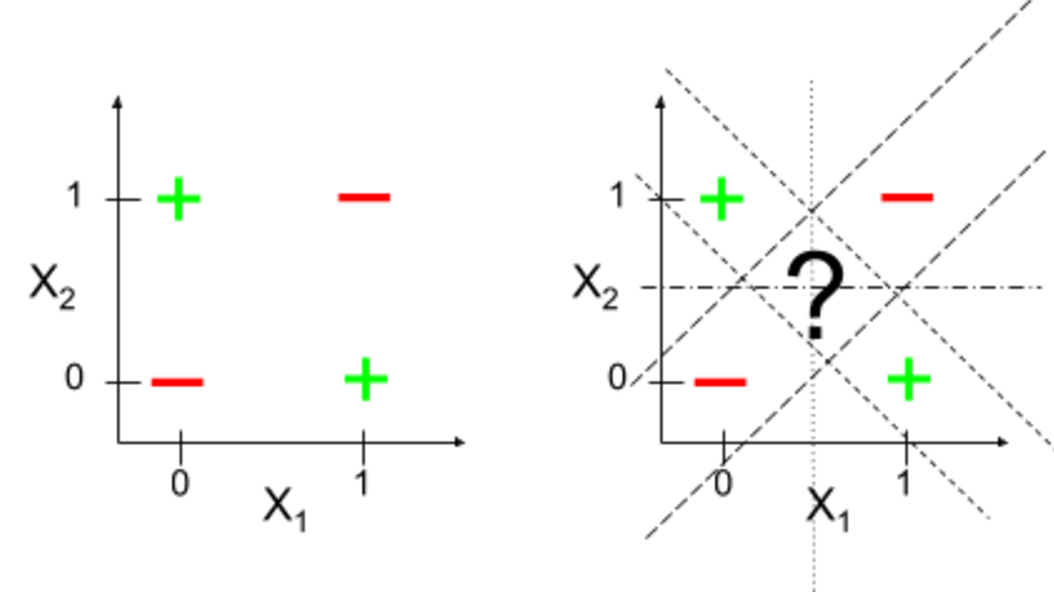
\includegraphics[scale=0.3]{obrazky-figures/xor.png}
    \caption{\label{fig:xor}Graf funkce XOR, jejíž výstup není lineárně separovatelný} 
\end{figure}





\section{Konvoluční neuronové sítě}
\todo{Nebo to pojmenovat jako Konvolucni vrstva?}.
Konvoluční neuronové sítě jsou typ feedforward sítí, které neobsahují pouze plně propojené vrstvy, ale také vrstvy konvoluční.
\begin{figure}[H]
    \centering
    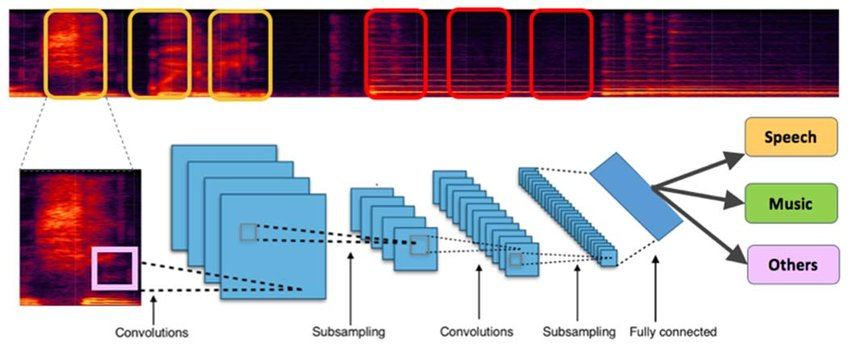
\includegraphics[scale=0.5]{obrazky-figures/conv_nn_audio.jpg}
    \caption{\label{fig:conv_nn}Konvoluční neuronové sítě}
\end{figure}

\subsection{Konvoluční vrstva}
Diskrétní konvoluce je definována jako

%\begin{equation}
%   (f * g)_k = \sum_{i=-\inf}^{\inf} f_i g_{k-i} = \sum_{i=-\inf}^{\inf} f_{k-i} g_{i}
%\end{equation}

kde $\star$ je konvoluční operátor, $f$ je funkce signálu, funkce $g$ je konvoluční jádro a $f_i$ a $g_i$ jsou hodnoty funkce na indexu $i$.



\section{Učení neuronových sítí}
Cílem trénování je naučit neuronovou síť vykonávat nějaký úkol. Trénování založené na metodě učení s učitelem vyžaduje dostatečně velký dataset obsahující dvojice vstup--výstup a obnáší volbu objektivní funkce, kterou se během trénování snažíme minimalizovat. 

Formálně je cílem učení aproximovat nějakou funkci $f^\ast$. Síti je předána vstupní hodnota $x$, pro kterou síť definuje mapování na výstupní hodnotu jako $y = f(x; \theta)$, kde $\theta$ je parametr, který se síť učí tak, aby dosáhla nejlepší aproximace funkce. \cite[p.~163]{mitdeeplearning}.


\subsection{Objektivní funkce}
Objektivní funkce (loss funkce, cost funkce) je funkce, která je během učení minimalizována nebo maximalizována, v závislosti na konkrétním úkolu a kontextu použití. Tato funkce mapuje událost či hodnoty na reálné číslo reprezentující \todo{spravit uvozovky} "cenu", která je asociována s touto událostí či hodnotami. Je--li tato funkce použita pro optimalizační problém, pak je cílem hodnotu minimalizovat a funkci se pak říká loss funkce, protože její výstupní hodnota nám udává velikost chyby, která se počítá na základě rozdílu mezi výstupem sítě a odpovídajícími trénovacími daty z datasetu.  

V rámci učení sítě je žádoucí, aby gradient objektivní funkce byl dostatečně velký (prudký) a předvídatelný. V takovém případě bude dobře sloužit pro účely trénování. V případě malého gradientu by funkce saturovala (byla by příliš plochá) a to by mohlo negativně ovlivnit trénování sítě \cite{mitdeeplearning}. 

Použije--li se hodnota objektivní funkce s opačným znaménkem, tak lze funkci použít jako hodnotící metriku. 


\subsection*{MSELoss (Mean Squared Error Loss)}
\todo{vzorecek a graf}
MSELoss je nejčastěji používaná objektivní funkce při řešení regresních problémů. Vypočítá se jako
\begin{equation}
  MSE = \frac{1}{N}\sum_{i=1}^N(y_i - \hat{y_i})^2
\end{equation}
kde $N$ je počet trénovacích dat v datasetu, $y_i$ je předpovězená hodnota a $\hat{y_i}$ je odhadnutá hodnota. Vzhledem k druhé mocnině je výsledek vždy pozitivní nezávisle na znaménku hodnot $y_i$ a $\hat{y_i}$. Druhá mocnina také zajišťuje, že čím větší je rozdíl mezi předpovídanou a aktuální odhadnutou hodnotou, tím více se chyba projeví.

\begin{figure}[H]
    \centering
    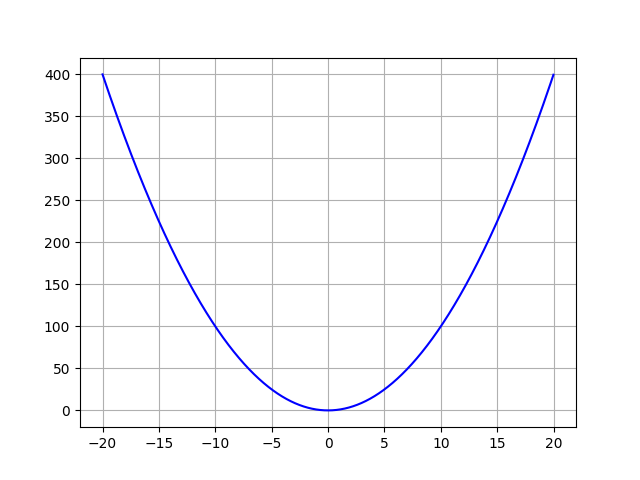
\includegraphics[scale=0.4]{obrazky-figures/mseloss.png}
    \caption{\label{fig:mseloss}Graf objektivní funkce MSE Loss}
\end{figure}

\subsection*{Cross Entrophy}
\todo{vzorecek}



\subsection{Backpropagation}
Backpropagation (backprop) je algoritmus typu učení s učitelem pro učení neuronových sítí. Algoritmus zpětně prochází neuronovou síťí a na základě hodnoty cost funkce $J(\theta)$ počítá její gradient metodou \textit{gradient descent}. Cílem je upravit všechny váhy v síti na základě toho, jak moc každá váha přispívá k celkové chybě. Algoritmus backpropagation počítá řetězové pravidlo (\textit{chain rule}).

Algoritmus se skládá ze 3 opakujících se kroků. Prvním krokem je forward fáze, ve které se počítá pro každou dvojici vstupu a referenčního výstupu 


\cite{web-brilliant}
\cite[p~197]{deeplearning}


- zpetne sireni chyby
- adaptacni algoritmus, podil neuronu na chybe,
- 3 opakujici se faze uceni:

1) feedforward - dopredu
2) zpetne sireni chyby - Backpropagation
3) uprava vah a biasu na zaklade chyby pomoci gradient descent
- chain rule



\subsection*{Gradient descent}
Gradient descent je iterativní optimalizační algoritmus pro hledání lokálního minima diferencovatelné objektivní funkce $J(\theta)$, kde $\theta \in \mathbb{R}^d$ reprezentuje učené parametry modelu, úpravou těchto parametrů v opačném směru, než je hodnota gradientu. Výpočet je prováděn postupným pohybem ve směru největšího klesání, které je určeno zápornou hodnotou gradientu. Rychlost pohybu závisí na velikosti kroku, což udává \textit{learning rate}. Správná volba \textit{learning rate} ovlivňuje rychlost, jakou je nalezeno minimum funkce. Při nízké hodnotě bude výsledek přesnější, ale nalezení minima bude výpočetně náročnější, protože v každém kroku se počítá nová hodnota gradientu. Při větší hodnotě je riziko, že minimum bude přeskočeno\cite{ruder2016overview}.
\begin{figure}[H]
    \centering
    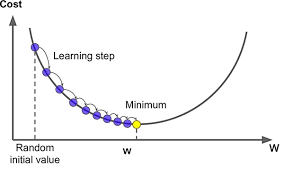
\includegraphics[scale=0.7]{obrazky-figures/gradientdescent.png}
    \caption{\label{fig:gradientdescent}Ukázka algoritmu gradient descent při hledání minima dané funkce postupným přibližováním dle nastavené velikosti kroku}
\end{figure}


\todo{popsat vice vliv LR na loss}


\subsection{Underfitting a generalizace}
Generalizace, neboli \textit{test error}, je vlastnost modelu, která udává, jak dobře model pracuje s dříve neviděnými daty, tedy s daty, které nebyly použity pro jeho učení. Během učení vzniká učící chyba, která je trénováním postupně minimalizována, ale kvalita modelu je pak měřena na testovacích datech. 
Testovací chyba by ideálně měla být co nejblíže chybě na trénovací sadě. Z rozdílu mezi těmito chybovými hodnotami se dají diagnostikovat problémy s naučením sítě -- podučení (\textit{underfitting}) a přeučení(\textit{overfitting}). 

\textit{Underfitting} nastane v případě, že model se již nedokáže v důsledku jeho kapacity zmenšit dostatečně jeho chybovou hodnotu na trénovacím datasetu.

\textit{Overfitting} nastane, když rozdíl mezi trénovací chybou a testovací chybou je příliš velký.

Kapacita je vlastnost modelu určující, kolik se toho dokáže model naučit. V případě nízké kapacity se model nedokáže naučit všechny příznaky z trénovacích dat a v případě vysoké kapacity se mohou přeučit zapamatováním si jejich příznaků a tím sice dosáhnou nízké trénovací chyby, ale špatných výsledků během testování\cite[p107]{mitdeeplearning}.
\begin{figure}[H]
    \centering
    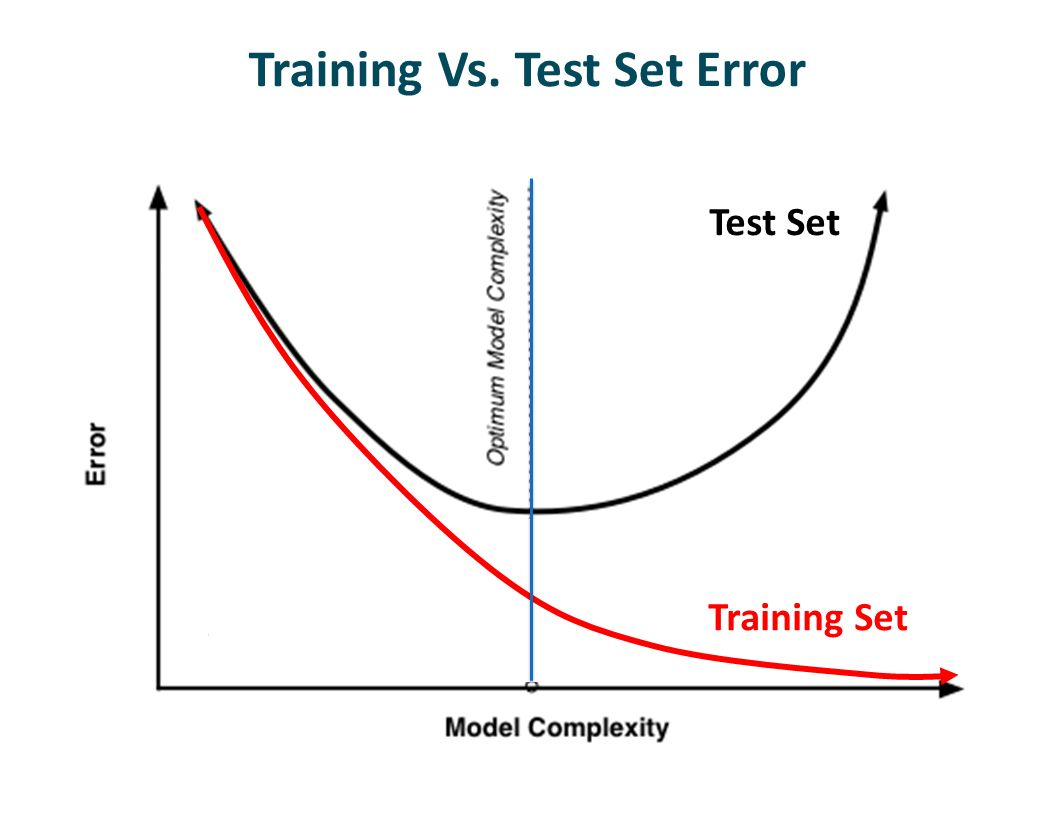
\includegraphics[scale=0.3]{obrazky-figures/capacity_vs_error.jpg}
    \caption{\label{fig:gradientdescent}Vliv kapacity modelu trénovací a testovací chybu}
\end{figure}


\subsection{Regularizace}
Regularizace je souhrn postupů, které říkají, jak modifikovat učící algoritmus tak, aby se zredukovala chyba generalizace, zatímco testovací chyba zůstane stejná\cite[p117]{mitdeeplearning}.


\subsection{Residuální spojení}
\todo{Toto chce obrazek residualniho spojeni. Popsat. Citovat odnekud, proc jsou residualni spojeni dobra pro trenovani DeepNN a v jednom odstavci to nejak shrnout}.


\subsection{Význam validační množiny v~trénování}
\todo{Mozna ne jako subsekci ale jen jako jeden odstavec}
Většina algoritmů strojového učení má nějakou sadu hyperparametrů, kterou je upravováno chování algoritmu. Hodnoty hyperparametrů obvykle bývají nastavovány ručně ještě před spuštěním procesu učení a hodnota se v~průběhu nemění, protože hodnoty by bylo obtížné optimalizovat. 
Některá nastavení se nicméně mohou stát hyperparametrem a být upravována během trénování, ale není vhodné je měnit na základě výsledku učení na trénovací sadě, protože by mohlo dojít k~přetrénováníoverfitting) v~důsledku \todo{CEHO??}. Pro tento případ potřebujeme validační sadu, která je odlišná od trénovací sady.
Po každém zpracování trénovací sady následuje validační sada, po jejímž skončení jsou optimalizovány hyperparametry[][].
\todo{[kniha 117-118] kap 5.3 = Hyperparameters and validation set} 
\todo{najit jeste nejakej zdroj s~popisem a pripadne nejaky zajimavejsi info.}



\todo{today mini zaver teto cele kapitoly}

%----------------------------------------------------------------------------------------------------------------------------------------------------------------------
%----------------------------------------------------------------------------------------------------------------------------------------------------------------------
\chapter{TasNet - Time--Domain Audio Separation Network}
\label{tasnet}

\todo{uvod do kapitoly}

\todo{Architektura full -- obrázek, bloky... Na zacatku zminit ze kapitola vychazi ze studie ref studie. Kapitola NEBUDE moc dlouha, cca 5-6 stran max.}

\begin{figure}[H]
    \centering
    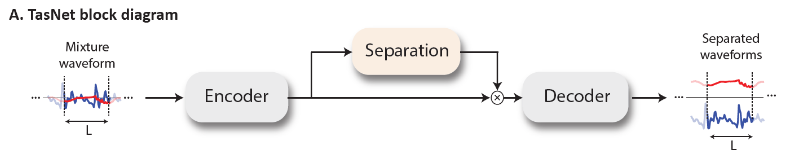
\includegraphics[scale=0.5]{obrazky-figures/tasnet-pipe.png}
    \caption{\label{fig:tasnet-pipe}Zjednodušený model architektury}
\end{figure}


\section{Konvoluční auto--enkodér}
\todo{Konvoluční autoenkodér, vstup, výstup...}

- schema bez separacniho modulu
- non negative representation of audio
\begin{figure}[H]
    \centering
    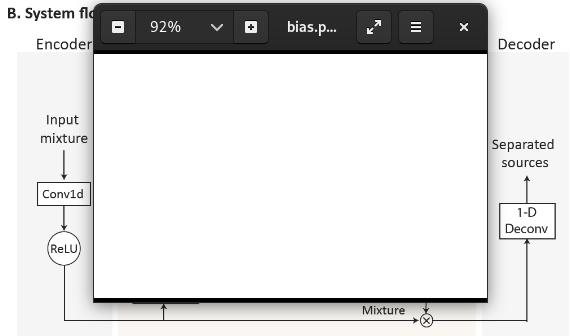
\includegraphics[scale=0.5]{obrazky-figures/tasnet-autoencoder.png}
    \caption{\label{fig:tasnet-autoencoder}Schéma konvolučního autoenkodéru}
\end{figure}


\section{Separační modul}
- odhad masek pro jednotlive mluvci
- schema se separacnim modulem
\begin{figure}[H]
    \centering
    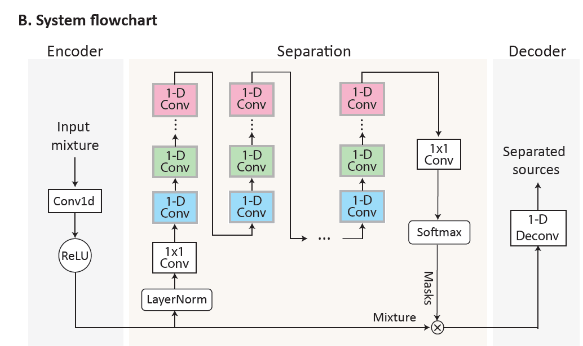
\includegraphics[scale=0.6]{obrazky-figures/tasnet-architecture.png}
    \caption{\label{fig:tasnet-modul}Schéma architektury TasNet}
\end{figure}


\subsection{Konvoluční bloky}
- Z~čeho se skládá -- konvoluční vrstvy, normalizace
- diagram konv bloku.
- Mozna: Dilatace a time perception
\begin{figure}[H]
    \centering
    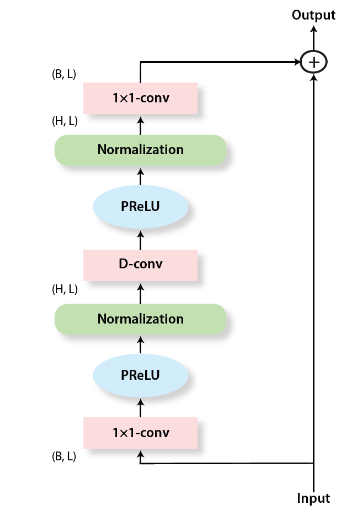
\includegraphics[scale=0.5]{obrazky-figures/conv-res-block.png}
    \caption{\label{fig:tasnet-convblock}Jeden konvoluční blok}
\end{figure}


\todo{zaver kapitoly}

%----------------------------------------------------------------------------------------------------------------------------------------------------------------------


\chapter{Implementace sítě}
\label{implementace}
Pro implementaci neuronových sítí vzniklo mnoho frameworků jako pytorch, tensorflow, keras a další, které umožňují síť poskládat z již předdefinovaných modulů. Jejich vlastnosti lze modifikovat dle potřeby pomocí argumentů při jejich instanciaci nebo při jejich použití. Kromě těchto bloků a mnoha dalších možností frameworky obsahují i metody pro práci s datasety, funkce pro vykreslování grafů a pro matematické operace.

Mým úkolem bylo implementovat neuronovou síť podle architektury TasNet pro separaci mluvčích v časové doméně. V rámci zadání jsem si zvolil použít framework s názvem pytorch\footnote{\url{https://pytorch.org/}}, který má kvalitní dokumentaci a aktivní uživatelskou základnu. Pytorch funguje nad jazykem Python\footnote{\url{https://www.python.org/}} a v celé práci používám jeho aktuálně nejnovější verzi (Python 3.8.2) a mimo jiné podporuje práci s datasety, včetně implementace vlastního nahrávání a manipulace s daty. Základní jednotkou, se kterou síť pracuje, je tensor. Ve frameworku pytorch je \textbf{torch.Tensor} třída reprezentující multidimenzionální matici obsahující data jednoho typu. Na tensory jsou převáděna data během načítání datasetu a následně předávána síti ke zpracování. Samotná implementace probíhala na systému Kali linux (4.19.0-kali5-amd64), který je založený na systému Debian. Aplikace byla vyvíjena v textovém editoru Vim\footnote{\url{https://www.vim.org/}} a byla během implementace spouštěna a testována v příkazovém procesoru Bash\footnote{\url{https://www.gnu.org/software/bash/}} (Bourne Again SHell) verze 5.0.16. Bash jsem zvolil i pro implementaci některých pomocných skriptů kvůli jednoduchému spouštění z terminálu a možnostem automatizace některých opakujících se příkazů. Pro správu verzí jsem používal verzovací systém Git\footnote{\url{https://git-scm.com/}}.

Trénování sítě probíhalo z~počátku na CPU \textit{intel i5} mého osobního notebooku \textit{Lenovo Y50-70}, což se ale ukázalo jako naprosto nevhodné vzhledem k náročnosti výpočtu kvůli nedostatečnému výkonu. Začal jsem tedy používat službu \textit{Google colab}, která poskytuje na omezenou dobu (12 hodin) stroje, které navíc obsahují technologii \textit{cuda}, což mi umožňilo výpočet provádět na GPU, čímž se trénování zrychlilo několikanásobně. Ještě více pomohlo předplacení služby, čímž se mi prodloužila doba, po kterou jsem mohl síť trénovat, na 24 hodin a zvýšila se šance na získání silnějších strojů. Modely byly trénovány na GPU \textit{T80} a \textit{T100} v závislosti na tom, která z nich mi zrovna byla přidělena pro dané sezení (\textit{session}). 

\bigskip
\todo{zamyslet se co tu chci ukazat v tom algu, pripadne vypustit parsovani, instanciaci atd}
\begin{algorithm}[H]
 \LinesNumbered
 parsování argumentů programu\;
 instanciace modelu TasNet\;
 \If{$args.checkpoint != NULL$}{
	načtení checkpointu\; 
 }
 instanciace třídy SegmentDataset a dataloaderu pro trénovací data\;
 instanciace třídy SegmentDataset a dataloaderu pro validační data\;
 \For{epocha v args.Epochs}{
  \tcc{trénování}
  loss = 0\;
  \For{směs\_mluvčích z trénovacího datasetu}{
    \tcc{cyklus načítá z dataloaderu segmenty nahrávek, které jsou generovány v třídě SegmentDataset}
  	$odhadovaná\_separace = TasNet(směs\_mluvčích)$\;
  	$loss = sisnr(optimální\_separace, odhadovaná\_separace)$\;
  	propagace chyby a úprava vah\;
  }
  \tcc{validace}
  vypnout gradient\;
  \For{směs\_mluvčích z validačního datasetu}{
  	$odhadovaná\_separace = TasNet(směs\_mluvčích)$\;
  	$validacni\_loss = sisnr(optimální\_separace, odhadovaná\_separace)$\;
  	\If{hodnota validační loss neklesla potřetí v řadě}{
		$learning\_rate = learning\_rate / 2$\;
  	}
  }
  na konci epochy uložit checkpoint\;
 }
 \caption{\label{alg:zakladnibeh}Zjednodušený algoritmus běhu programu pro trénování sítě}
\end{algorithm}

%------------------

\section{Implementace modelu}
\todo{today DNES - miniuvod k implementaci modelu - nic podrobneho, je to uz zmineno predtim ze to je v pytorchi atd}
\todo{Pozn: pytorch, scripty, tridy, moduly, parametry a volby spusteni}


Model se skládá ze separační části, která se skládá z konvolučních bloků, dále z...



\subsection*{Třídy SegmentDataset a AudioDataset}
\todo{zpracovani datasetu, jedna segmentuje, druha ne}
Blizsi popis segmentace v podkapitole \ref{sec:segmentace}.

%------------------

\subsection*{Třída Tasnet}
Třída Tasnet.py reprezentuje model neuronové sítě. Atributy třídy představují jednotlivé vrstvy neuronové sítě. Síť obsahuje konvoluční vrstvy, enkodér, dekodér a \textit{temporal convolutionan network}, která je tvořena sekvencí konvolučních bloků, které jsou zmíněny dále. V této třídě jsou také inicializovány váhy algoritmem xavier\todo{citovat}. Ve funkci $forward()$, která je volána, když jsou instanci sítě předána data ke zpracování, jsou sekvenčně volány jednotlivé vrstvy. Během zpracování předaných dat je v této sekvenci vypočítána maska a aplikována na zpracovávanou směs. Tím vzniknou dvě separované nahrávky, které jsou předány na výstup. 
\todo{zminit stride, padding, a mozna obrazek co to je a mozna trochu prepsat (ktere, ktera, ktere).}

%------------------

\subsection*{Třída ResBlock}
Třída ResBlock reprezentuje jeden konvoluční blok, který je opakován se zvyšující se dilatací v \textit{temporal convolutional network} v separační části určené k odhadu masek. Podobně jako třída Tasnet, i tato třída obsahuje inicializaci a zřetězení vrstev. V inicializaci jsou nastaveny hodnoty pro konvoluční operace jako počet konvolučních jader, časová dilatace a počet kanálů. Tyto operace jsou ve funkci \textit{forward} zřetězeny do sekvence konvolučních operací a aktivačních funkcí, podle vzorové architektury TasNet. Třída ResBlock je specifická svým residuálním spojením, kde dochází k rozdělení dat při zpracování, kdy jedna kopie je transformována operacemi v bloku a na konci sečtena s daty, které transformacemi neprošly a tento součet je výstupem bloku. Residuální spojení jsou podrobněji popsána v kapitole \ref{neuronovky}.

%------------------------------------------------------

\section{Segmentace nahrávek}
\label{sec:segmentace}
Pro účely trénování sítě byly vstupní nahrávky rozdělovány na segmenty o délce 4, případně 2 sekund. Délku segmentů $L_s$ lze nastavit přes argument $\texttt{----segment\_length}$ při volání skriptu $train.py$. Tato hodnota reprezentuje jeden z hyper--parametrů sítě. Výchozí hodnota je 4 sekundy. Při nižších hodnotách se prodlužuje délka trénování, protože se z jedné vstupní nahrávky o délce $L$ vygeneruje až $L/L_s$  segmentů a tím narůstá počet dat, který síť musí zpracovat. 

Poslední segment by byl kratší, pokud by délka nahrávky byla kratší než délka segmentu. V takovém případě je segment doplněn nulami do délky ostatních segmentů jak lze vidět na obrázku \ref{fig:segmentace_padding}. Toto doplnění je nutné kvůli dávkovému zpracování (\textbf{batches}), které neumožňuje rozdílnou délku elementů v dávce. Pokud je délka nahrávky delší než délka segmentu, tak se poslední segment vezme od konce bez nutnosti ho pak nulami doplňovat. Skládání segmentů do minibatche zobrazuje obrázek \ref{fig:minibatch_segmentace}. Při vzorkovací frekvenci $f_s = 8000Hz$, obsahují segmenty $f_s * L_s$ vzorků vstupní nahrávky. 

\begin{figure}[H]
    \centering
    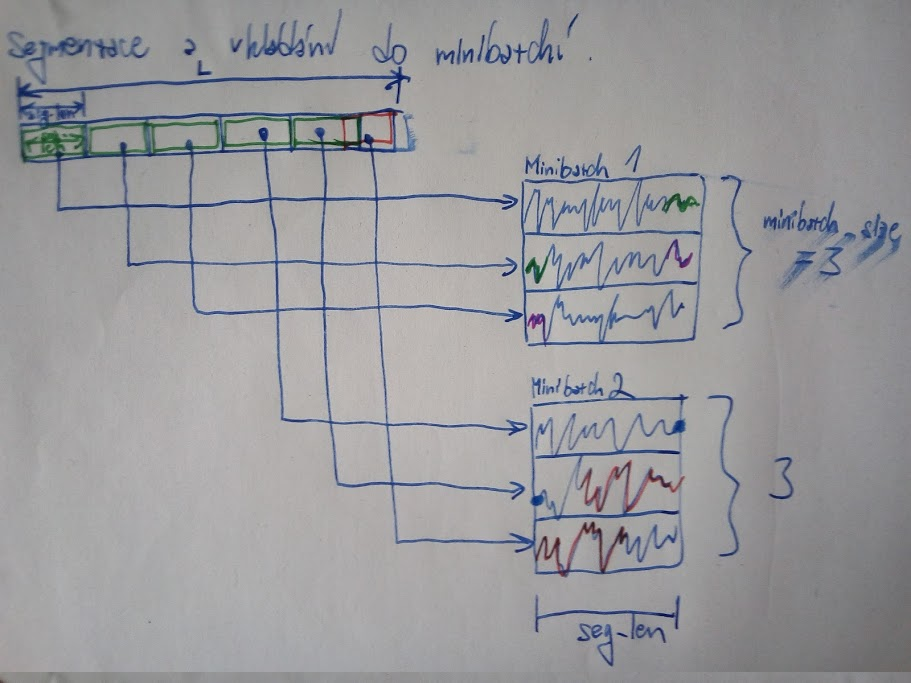
\includegraphics[scale=0.30]{obrazky-figures/minibatch_segmentace.jpg}
    \caption{\label{fig:minibatch_segmentace}Dělení nahrávky na segmenty o délce \textbf{segment\_len} a jejich následné vkládání do minibatche. Lze si všimnout, že pokud poslední segment není dostatečně dlouhý, tak se vezme od konce nahrávky a jeho počáteční vzorky budou duplicitní s posledními vzorky předešlého segmentu}
\end{figure}

\begin{figure}[H]
    \centering
    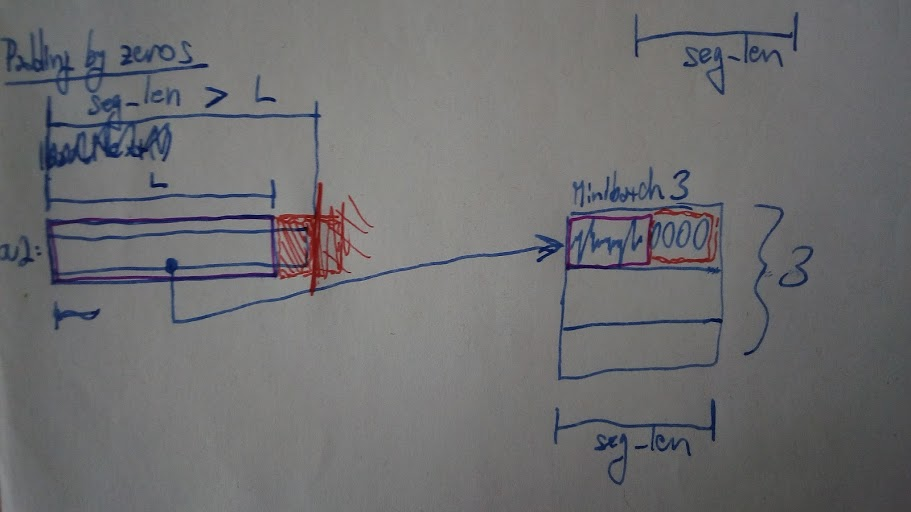
\includegraphics[scale=0.30]{obrazky-figures/minibatch_segmentace_padding.jpg}
    \caption{\label{fig:segmentace_padding}Je--li zpracovávána nahrávka, jejíž délka je kratší než je délka segmentu, je tento segment doplněn z prava nulami do požadované délky}
\end{figure}

\todo{mozna tento odstavec jeste nejak upravit a doplnit obrazek kde je nacitani asi 3 audio nahravek}
Algoritmus \ref{alg:segmentace_nahravek} a obrázek \ref{fig:generovani_segmentu} zobrazují proces segmentace. Funkce $\texttt{segmentGenerator()}$, která slouží jako generátor, pracuje současně se třemi nahrávkami -- se směsí dvou mluvčích, s nahrávkou prvního mluvčího a s nahrávkou druhého mluvčího, které jsou do atributů $\texttt{current\_mixture}$, $\texttt{current\_source1}$ a $\texttt{current\_source2}$ třídy $\texttt{SegmentDataset}$ nahrávány funkcí $\texttt{loadNextAudio()}$ poté, co z předchozí trojice nahrávek již nelze vygenerovat další segmenty.

\bigskip

\begin{algorithm}[H]
\LinesNumbered
\SetKwProg{Fn}{Function}{ is}{end}
 \Fn{segmentGenerator() : int[]}{
	 $\texttt{s1\_segment} = \texttt{[]}$\;
	 $\texttt{segptr} = \texttt{0}$\;
	 \While{$\texttt{je dostupná další trojice nahrávek}$}{
		\eIf{$\texttt{current\_mixture\_len} < \texttt{SEGMENT\_LENGTH}$}{
			\tcc{aktuální nahrávka je kratší než délka segmentu}
			$\texttt{s1\_segment} = \texttt{current\_source1[:]}$\;
			$\texttt{yield s1\_segment}$\;
		}{
			\eIf{$\texttt{segptr} + \texttt{SEGMENT\_LENGTH} < \texttt{current\_mixture\_len}$}{
				\tcc{z aktuální nahrávky vzít segment}				
				$\texttt{s1\_segment} = \texttt{current\_source1[(segptr+SEGMENT\_LENGTH)]}$\;
				$\texttt{segptr} += \texttt{SEGMENT\_LENGTH}$\;
				$\texttt{yield s1\_segment}$\;
			}{
				\tcc{nelze již načíst celý segment, takže se vezme od konce}
				$\texttt{start\_index} = \texttt{(current\_mixture\_len - SEGMENT\_LENGTH)}$\;
				$\texttt{s1\_segment} = \texttt{current\_source1[start\_index:current\_mixture\_len]}$\;
				$\texttt{yield s1\_segment}$\;
			}
		}
	}
 }
 \caption{\label{alg:segmentace_nahravek}Algoritmus segmenace nahrávek používá výhody python generátoru, který, narozdíl od běžných funkcí, po vrácení hodnoty příkazem \texttt{yield} neztrácí svůj vnitřní stav a při jeho dalším zavolání pokračuje tam, kde skončil. V uvedeném příkladě je znázorněna pouze segmentace nahrávky jednoho mluvčího, ale analogicky se segmentují i nahrávky směsi mluvčích a nahrávky druhého mluvčího}
\end{algorithm}


\begin{figure}[H]
    \centering
    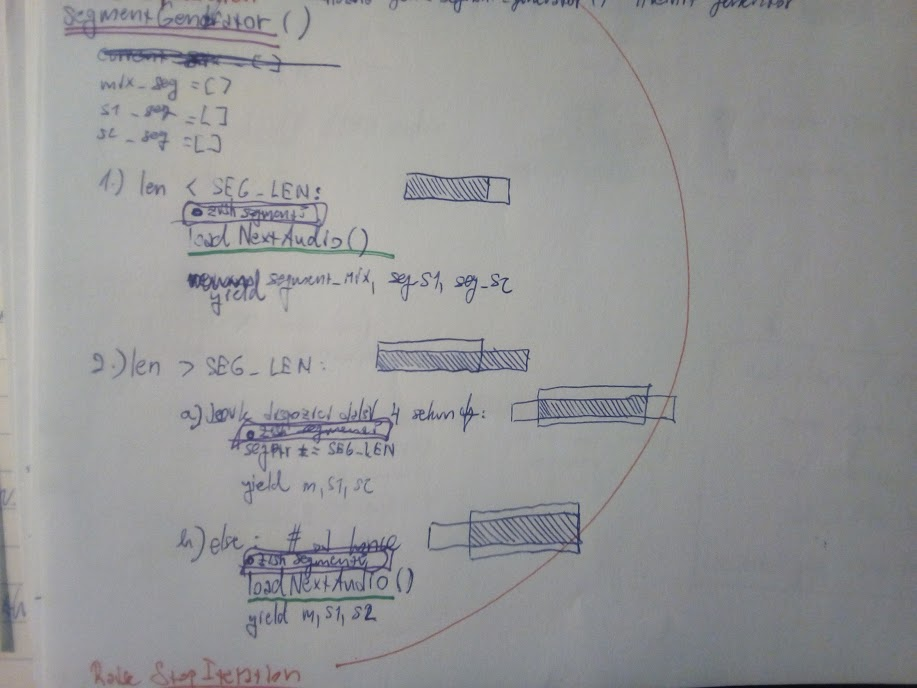
\includegraphics[scale=0.30]{obrazky-figures/segmentation.jpg}
    \caption{\label{fig:generovani_segmentu}Způsob segmentace nahrávek}
\end{figure}


Kód segmentace také umožňuje určit délku, o kterou se segmenty budou překrývat. Této funkcionality je docíleno zavedením proměnné \texttt{overlap}, která obsahuje délku překrytí a při segmentaci je od proměnné \texttt{offset}, který určuje začátek následujícího segmentu, tato hodnota odečtena, jak ukazuje obrázek \ref{fig:segment_overlap}. Při trénování je překrytí nulové, protože by to zvýšilo počet trénovacích dat jejich částečnou duplikací, což by negativně ovlivnilo délku trénování.

\begin{figure}[H]
    \centering
    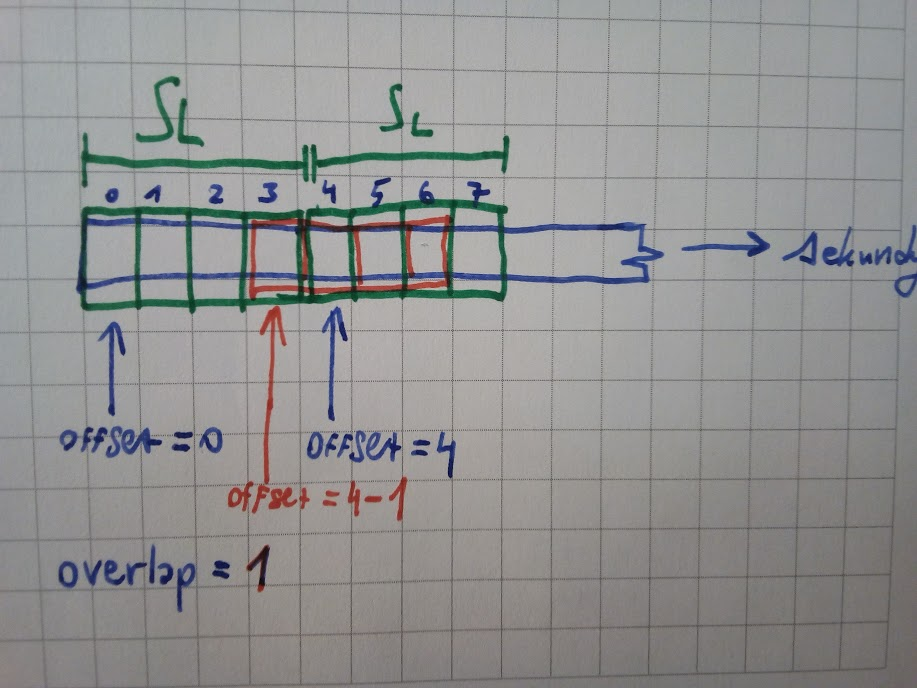
\includegraphics[scale=0.25]{obrazky-figures/segment_overlap.jpg}
    \caption{\label{fig:segment_overlap}Segmentace nahrávek s nenulovým překrytím}
\end{figure}

%------------------
\section{Výpočet hodnoty loss za pomoci si--snr}
\todo{popsat implementaci sisnr a vypocet loss za pomoci cross vypoctu, obrazek}

\begin{figure}[H]
    \centering
    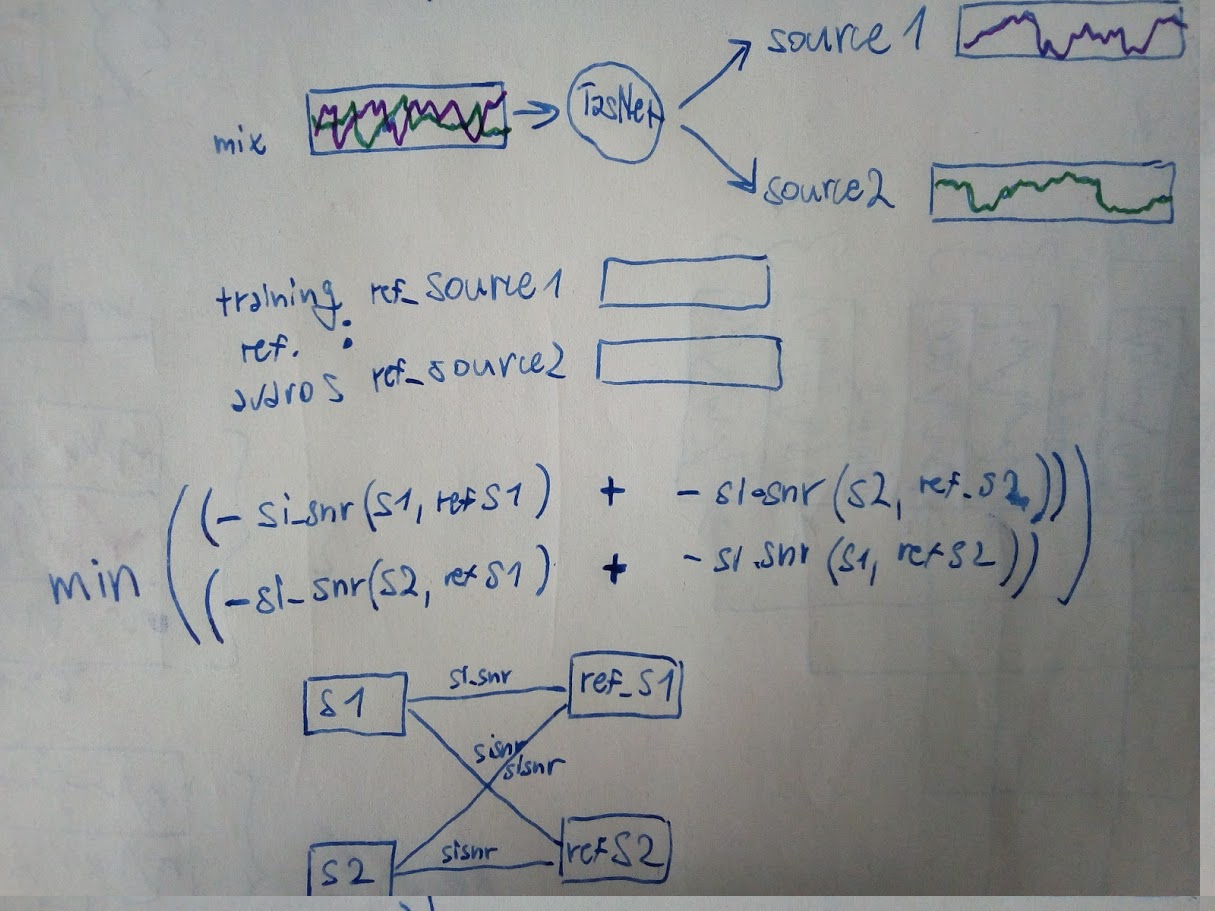
\includegraphics[scale=0.25]{obrazky-figures/sisnr_cross_calculation.jpg}
    \caption{\label{fig:implementace_loss_sisnr} Implementace a zjištění správné pozice korespondujících nahrávek pro výpočet hodnoty loss}
\end{figure}

%------------------
%------------------


\section{Pomocné skripty}
Během implementace se vyskytla potřeba zjednodušit si některé repetetivní úkony a jelikož upřednostňuji práci z terminálu, tak jsem si pro ně naprogramoval několik skriptů za použití jazyků python3 a bash. 

Skript \textbf{\textit{gupload.sh}} pro odesílání zdrojových souborů na \textit{Google Drive}\footnote{\url{https://www.google.com/drive/}}, ze kterého \textit{Google Colab}\footnote{\url{https://colab.research.google.com/notebooks/intro.ipynb}} načítá data a kód, který lze následně po částech spouštět z grafického rozhraní. K interakci s Google Drive jsem použil nástroj \textit{rclone}\footnote{\url{https://rclone.org/}}, který nabízí mnoho operací pro vzdálenou práci s Google Drive z terminálu. S pomocí \textit{rclone} lze stahovat či nahrávat data, vzdáleně měnit adresářovou strukturu, mazat, vytvářet a upravovat soubory a podobně. 

Skript \textbf{\textit{gdownload.sh}} je určený pro snadné stahování dat z Google Drive. Stejně jako předchozí skript, používá operace poskytované nástrojem rsync. Při zavolání stáhne adresář obsahující data z posledního trénování, nebo adresář, jehož název je předán jako argument skriptu v přikazové řádce.   
Stažený adresář obsahuje checkpointy, soubory obsahující výstup trénování, soubor obsahující dvojice hodnot $[zpracováno_nahrávek, loss]$, které lze jednoduše vykreslit do grafu, a nakonec soubor s výsledky testování obsahující hodnoty metrik pro testovaný checkpoint.

Dále jsem vytvořil několik jednoduchých skriptů pro rychlé spuštění trénování a testování modelu s různými přednastavenými parametry. Bylo tak možno mít mezi skripty rozdílné cesty k adresářům pro účely trénování a ladění chyb nebo třeba nastavení času, po kterém se proces má sám ukončit. Pro spuštění trénování modelu tak lze zavolat skript \textbf{\textit{nntrain.sh}}, pro testování skript \textbf{\textit{nntest.sh}} a pro inferenci (separaci mluvčích na předané nahrávce) skript \textbf{\textit{nninference.sh}}.


\bigskip

Implementace samotného modelu ve frameworku pytorch nebyla náročná. Vzhledem k netriviálnímu úkolu jsem musel implementovat některé části, jako třeba segmentace nahrávek, sám. To přineslo mnoho potíží při odstraňování chyb v samotném modelu. Síť jsem prvně trénoval a ladil na CPU svého notebooku, takže probíhalo velmi pomalu (v řádu desítek hodin i při nízké velikosti modelu), a některé chyby se objevily až v průběhu trénování nebo dokonce na jeho konci. Situaci razantně zlepšil přechod na Google Colab, kde jsem síť trénoval na poskytovaných GPU a trénování tak zabralo \todo{"pouze" (opravit uvozovky)} několik hodin, takže se případná chyba objevila dříve, ale i přesto mi lazení sítě zabralo mnoho času. Pro další usnadnění samotné implementace jsem vytvořil několik skriptů, které mi usnadnily spouštění a lazení sítě.

%----------------------------------------------------------------------------------------------------------------------------------------------------------------------


\chapter{Experimenty a vyhodnocení}
\label{experimenty}
- trenovani s~ruznymi hyperparametry, uspesnost a tabulky s~hyper parametry a dosazenymi vysledky a hodnotami sisnr, sdr atd.
- model size comparison.
- porovnani s~vysledky ze studie
- obrazky separovanych mluvcich - signalu.
- spektra
- grafy trenovani loss a vysledkuu.
- pametova narocnost modelu


Neuronové sítě představují mocný nástroj mnoha využití, který ale musí být naučen, jak danou činost provádět. Trénování sítí je výpočetně náročný úkol, jehož náročnost se, krom dalších parametrů, může lišit v závislosti na velikosti datasetu a sítě. Obecně čím větší dataset a rozměr sítě, tím déle trénování trvá. Je proto podstatné, na jakém stroji je síť učena a od toho se odvíjí čas trénování.

Po dostatečném natrénování probíhá vyhodnocení sítě. Výsledky trénování jsou měřeny metrikami, které se volí na základě problému, který se síť učila řešit. Výsledky testování sítě jsou následně porovnávány v závislosti na velikosti daného modelu. Velikost modelu je ovlivněna hyper--parametry, které určují například počet vrstev sítě, velikost segmentace a další vlastnosti.

Cílem experimentů je zjistit, které z hyper--parametrů mají největší vliv na kvalitu separace a tedy na výsledky vyhodnocení, a jak moc lze model zmenšit, aby stále dával dostatečně dobré výsledky separace mluvčích. Tato kvalita je měřena primárně metrikami STOI, SI--SNR a PESQ, které byly popsány v kapitole \ref{separace}.
\todo{ref na zdroje u metrik}


\section{Dataset}
Dataset je množina dat, na kterých je síť učena a testována. Dataset se dá rozdělit na 3 podmnožiny, které jsou navzájem exkluzivní. Trénovací dataset je určen k trénování sítě a bývá největší. Validační dataset se prochází po zpracování trénovacího datasetu v průběhu trénování a slouží pro ověření, že hodnota loss na dosud neviděných datech stále klesá a nedochází tak k přetrénování. Při zpracování tohoto datasetu je síti zabráněno v učení. Poslední je testovací dataset, na kterém probíhá vyhodnocení sítě, tedy výpočet hodnot jednotlivých metrik. 

Trénování a vyhodnocení modelu proběhlo na množině jednokanálových nahrávek směsí dvou mluvčích. Množina byla vygenerována náhodným výběrem různých mluvčích z~Wall Street Journal (WSJ0) a vytvořením směsi mluvčích z těchto dvou náhodně vybraných nahrávek. Celková délka trénovacích dat je přes 10 hodin a přes 6 hodin validačních dat. Nahrávky jsou převzorkovány na 8kHz a během trénování zarovnány na zero means a jednotkovou varianci \todo{[studie str 5 Dataset][49 - ze studie odkaz na script na generovani a popis na netu]}.

\begin{figure}[H]
    \centering
    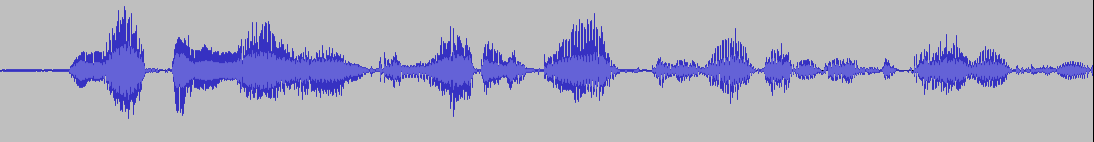
\includegraphics[scale=0.35]{obrazky-figures/dataset-mix.png}
    \caption{\label{fig:ref-mixture}Ukázka nahrávky směsi dvou mluvčích}
\end{figure}

\begin{figure}[H]
    \centering
    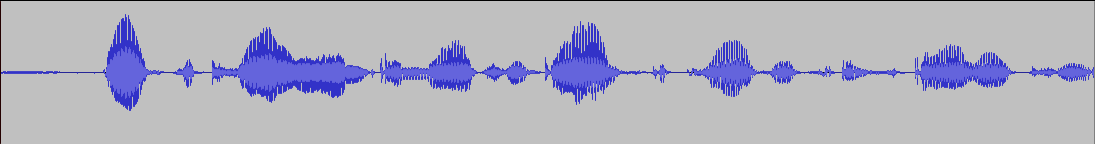
\includegraphics[scale=0.35]{obrazky-figures/dataset-s1.png}
    \caption{\label{fig:ref-s1}První mluvčí ze směsi}
\end{figure}

\begin{figure}[H]
    \centering
    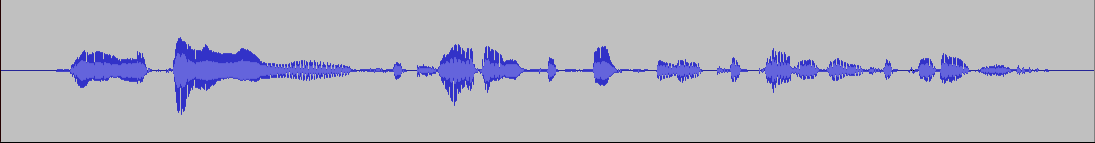
\includegraphics[scale=0.35]{obrazky-figures/dataset-s2.png}
    \caption{\label{fig:ref-s2}Druhý mluvčí ze směsi}
\end{figure}

Lze si všimnout, že sečtením signálů separovaných mluvčích na obrázku \ref{fig:ref-s1} a \ref{fig:ref-s2} dostaneme přesně signál směsi, což lze vyjádřit vztahem

\begin{equation}
  x[t] = \sum_{i=1}^C s_i[t]
\end{equation}
, kde $x[t] \in \mathbb{R}^{1 \times T}$ je diskrétní signál směsi a $s_i[t] \in \mathbb{R}^{1 \times T}$, kde $i = 1,\ldots,C$, je jeden z~$C$ zdrojů[cite studie str3 vlevo]. 

\todo{doplnit info o~zero means a jendotkove varianci}


%------------------------------------------------------------------------------


\section{Průběh trénování}
\todo{miniÚvod - konkretni hyperparams, vykon a cas trenovani, seg--len, bylo natrenovano nekolik modelu ... konkretni hyperparams, vykon a cas trenovani, seg--len}.
Bylo natrénováno několik, různě velkých modelů, které se lišily velikostí jejich hyper--parametrů, konkrétně počtem konvolučních bloků, počtem jejich opakování a velikostí segmentů zpracovávaných nahrávek z datasetu. 

\todo{https://www.tablesgenerator.com/}.

\begin{table}[hbt]
\centering
\caption{Hodnoty hyperparametrů trénovaných sítí a jejich přesnost}
\label{hodnoty}
\begin{tabular}{|l|c|c|c|}
\hline
 & X & R & segment length  \\
 &  &  & sisnr  \\ \hline
2 & 2 & 4 & 8.3 \\ \hline
3 & 2 & 4& 9.45 \\ \hline
4 & 3 & 4 & 10.2 \\ \hline
8 & 4 & 2 & 13.6 \\ \hline
\end{tabular}
\end{table}


\begin{figure}[H]
    \centering
    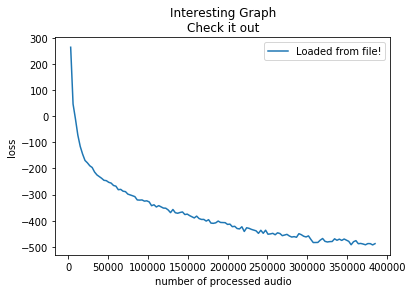
\includegraphics[scale=0.55]{obrazky-figures/some-loss.png}
    \caption{\label{fig:somelossTODO}Příklad grafu loss hodnoty během učení}
\end{figure}

\begin{figure}[H]
    \centering
    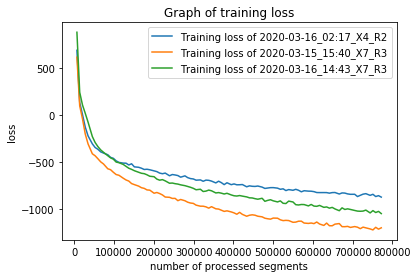
\includegraphics[scale=0.55]{obrazky-figures/loss_triple.png}
    \caption{\label{fig:somelossTODO2}Hodnota loss při trénování modelů s~různou velikostí hyperparametrů}
\end{figure}


%------------------------------------------------------------------------------

\section{Experimenty s modely}
\todo{rozdelit tabulku podle HP a spis mensi tabulku ukazujici vysledku pro konkretni hyper parametry.
experimenty:
sisnr, reportovat ruzne metriky - stoi, pesq, prozkoumat hyper parametry a jak ktere jsou dulezite. Kdyz budu zmensovat sit tak jak se bude zhorsovat.}

\todo{miniÚvod}
Pro vyhodnocení úspěšnosti a kvality modelů byly použity metriky si--snr vyjadřující poměr XXX, pesq říkající YYY a stoi vyjadřující ZZZ \todo{mozna ref}.  

\subsection{Vliv hyper--parametru X}
\todo{zmensovani a zvetsovani X, vysledky testovani, loss pripadne nejake fajnove grafy porovnani vysledky mezi jednotlivymi X, obrazky, grafy}

\subsection{Vliv hyper--parametru R}
\todo{zmensovani a zvetsovani Y, vysledky testovani, loss pripadne nejake fajnove grafy porovnani vysledky mezi jednotlivymi Y, obrazky, grafy}

\subsection{Vliv hyper--parametru délka--segmentu}
\todo{zmensovani a zvetsovani SL, vysledky testovani, loss pripadne nejake fajnove grafy porovnani vysledky mezi jednotlivymi SL, obrazky, grafy}

\subsection{Vyhodnocení a porovnání modelů}
\todo{shrnuti a porovnani jednotlivych zmen mezi sebou komplexne. Pripadne porovnani vysledku s ref studii, obrazky, grafy}




\section{Možná rozšíření a navrhnutá vylepšení}
- variabilnější dataset, mikrofony, šum a bordel prostředí
- separace více mluvčích
- hlučné prostředí
- identifikace konkrétního řečníka
- realtime separace

%----------------------------------------------------------------------------------------------------------------------------------------------------------------------
%----------------------------------------------------------------------------------------------------------------------------------------------------------------------

\chapter{Závěr}
\label{zaver}
\todo{co jak dopadlo, vysledky a vyhodnoceni velikosti modelu a jaky byl nejlepsi}

Cílem práce bylo implementovat síť podle architektury TasNet pro separaci mluvčích v~časové doméně a porovnat vliv velikosti sítě na kvalitu separace. Síť byla implementována za pomoci frameworku pytorch a jazyku python a natrénována na datasetu obsahujícím jednokanálové směsi dvou mluvčích. Trénování proběhlo na \todo{X} modelech, které se od sebe lišily počtem opakujících se konvolučních bloků, velikostí časové dilatace a délkou vstupních segmentů směsí. Pro účel vyhodnocení modelů byla použita metrika si-snr, která udává poměr chtěného signálu ku šumu na pozadí, tedy obecně kvalitu separace. 

Experimenty ukázaly, že během testování nejlépe dopadla síť, která měla 8 konvolučních bloků po 4 opakováních, s~délkou vstupního segmentu $L=2$ sekundy. Tento model dosáhl po 100 epochách trénování hodnoty až \todo{13,4} a tím se stal nejúspěšnějším modelem. Při fyzickém poslechu separovaných nahrávek bychom neslyšeli téměř žádný náznak druhého mluvčího. Oproti tomu, nejméně přesný model měl pouze 4 konvoluční bloky, 2 opakování a při délce segmentů $L=4$ sekundy dosahoval hodnoty SDR pouze \todo{9.2}.

Zkoušel jsem separovat také nahrávky, které byly úplně mimo dataset, ale výsledek se nedá hodnotit jako úspěšný, jelikož hraje velkou roli prostředí, mikrofon, šum v~pozadí a další vlivy, na které byla neuronová síť naučena. Tento problém by se dal překonat rozšířením trénovacího datasetu o~větší škálu nahrávek mluvčích, které by byly pořízeny z~různých zařízení v~různě rušném prostředí.

\todo{Doplnit ještě neco eh}
Mozna.


